\documentclass{article}
\usepackage[utf8]{inputenc}
\usepackage{authblk}
\usepackage{setspace}
\usepackage[margin=1.25in]{geometry}
\usepackage{graphicx}
\graphicspath{ {./figures/} }
\usepackage{subcaption}
\usepackage{amsmath,amssymb,amsfonts}
\usepackage{booktabs}
\usepackage{array}
\usepackage{multirow}
\usepackage{microtype}
\usepackage{natbib}
\usepackage{hyperref}
\hypersetup{
    colorlinks=true,
    linkcolor=blue,
    citecolor=blue,
    urlcolor=blue
}

\title{\textbf{Order Book Imbalance and Contemporaneous Price Impact in Vietnamese Equities}}
\author[1*]{AI Quantitative Research Network}
\affil[1]{Autonomous Financial Machine Learning \& Empirical Econometrics Lab, Ho Chi Minh City, Vietnam}
\affil[*]{Contact: \texttt{research@vnresearch.org}}
\date{\today}
\onehalfspacing

\begin{document}
\maketitle

\begin{abstract}
\noindent \textbf{Hypothesis Formulation:} Tests whether daily order book supply/demand volume imbalance (OIR) exerts contemporaneous price impact and generates forward return drift in Vietnamese equities ($H_0: \beta_{\text{OIR}} = 0$ versus $H_1: \beta_{\text{OIR}} > 0$). \\
\textbf{Data \& Empirical Setting:} Daily order book bid/offer queue statistics (\path{vn_order_supply_demand_daily.parquet}) and VN-Index returns (\path{vn_indices_daily.parquet}) across 1,316 sessions from July 2021 to October 2026. \\
\textbf{Econometric Methodology:} Standardized market-wide order imbalance ratio $\text{OIR}_t = (V_{B,t} - V_{S,t}) / (V_{B,t} + V_{S,t})$, ADF stationarity tests, Newey--West HAC robust covariance estimation with Bartlett kernel lag selection ($L = 7$), and quintile portfolio sorting. \\
\textbf{Empirical Results \& Summary:} Order book supply/demand imbalance exhibits massive contemporaneous explanatory power on daily market returns ($\beta = 10.1043$, HAC $t = 11.4579$, $p < 10^{-29}$, $R^2 = 20.58\%$). Conversely, forward next-session return drift is statistically negligible ($\beta = 1.2336$, $t = 1.0926$, $p = 0.2746$). \\
\textbf{Research Decision:} \textbf{ACCEPTED (Contemporaneous Price Impact Confirmed)}. Limit order queue imbalances are contemporaneously absorbed into closing prices with near-complete informational efficiency.
\end{abstract}

\vspace{0.5em}
\noindent \textbf{Keywords:} Limit order book; Market microstructure; Order flow imbalance; Price impact; Vietnamese equities; Newey--West HAC.

\vspace{0.5em}
\noindent \textbf{JEL Classification Codes:} G14, G12, C22, D47.

\section{Introduction and Hypothesis Formulation}
\label{sec:intro}
In continuous double auction markets, queue size differences between the best bid and ask reflect incoming order flow pressure \citep{kyle1985continuous, chordia2002order}. We test whether aggregate order book volume imbalance contemporaneously shifts index returns ($H_0^{(1)}: \beta = 0$) and whether imbalances generate multi-day return drift ($H_0^{(2)}: \beta_{\text{next}} = 0$).

\section{Data and Econometric Methodology}
\label{sec:methods}
The empirical series are extracted from \path{data/market/vn_order_supply_demand_daily.parquet} and \path{data/market/vn_indices_daily.parquet}. We estimate:
\begin{align}
    r_t &= \alpha_1 + \beta_1 \cdot \text{OIR}_t + \varepsilon_t \\
    r_{t+1} &= \alpha_2 + \beta_2 \cdot \text{OIR}_t + \gamma \cdot r_{t-1} + \eta_{t+1}
\end{align}
Inference is conducted using Newey--West HAC standard errors \citep{newey1987simple}.

\section{Empirical Results}
\label{sec:results}
Table \ref{tab:order_flow_regressions} presents the estimation results.

\begin{table}[htbp]
\centering
\caption{Order Book Imbalance and Price Impact Regressions with Newey--West HAC Inference}
\label{tab:order_flow_regressions}
\resizebox{\textwidth}{!}{%
\begin{tabular}{lccccc}
\toprule
\textbf{Model / Specification} & \textbf{Coefficient ($\beta$)} & \textbf{HAC Std. Err.} & \textbf{$t$-Statistic} & \textbf{$p$-Value} & \textbf{$R^2$} \\
\midrule
\textbf{Model 1: Contemporaneous Price Impact ($r_t$)} & & & & & \\
Intercept ($\alpha$) & 0.4211 & 0.0450 & 9.36 & 0.0000 & -- \\
Order Imbalance Ratio ($\text{OIR}_t$) & 10.1043 & 0.8819 & 11.46 & 2.1456e-30 & 0.2058 \\
\midrule
\textbf{Model 2: Next-Session Predictability ($r_{t+1}$)} & & & & & \\
Intercept ($\alpha$) & 0.0786 & 0.0576 & 1.37 & 0.1719 & -- \\
Order Imbalance Ratio ($\text{OIR}_t$) & 1.2336 & 1.1290 & 1.09 & 0.2746 & -- \\
Lagged Return ($r_{t-1}$) & -0.0302 & 0.0380 & -0.79 & 0.4268 & 0.0049 \\
\bottomrule
\end{tabular}
}
\end{table}


Model 1 demonstrates that order imbalance explains 20.6\% of market return variance ($\beta = 10.1043$, $t = 11.46$, $p < 10^{-29}$). Figure \ref{fig:order_flow_plot} illustrates the regression fit and quintile portfolio returns.

\begin{figure}[htbp]
\centering
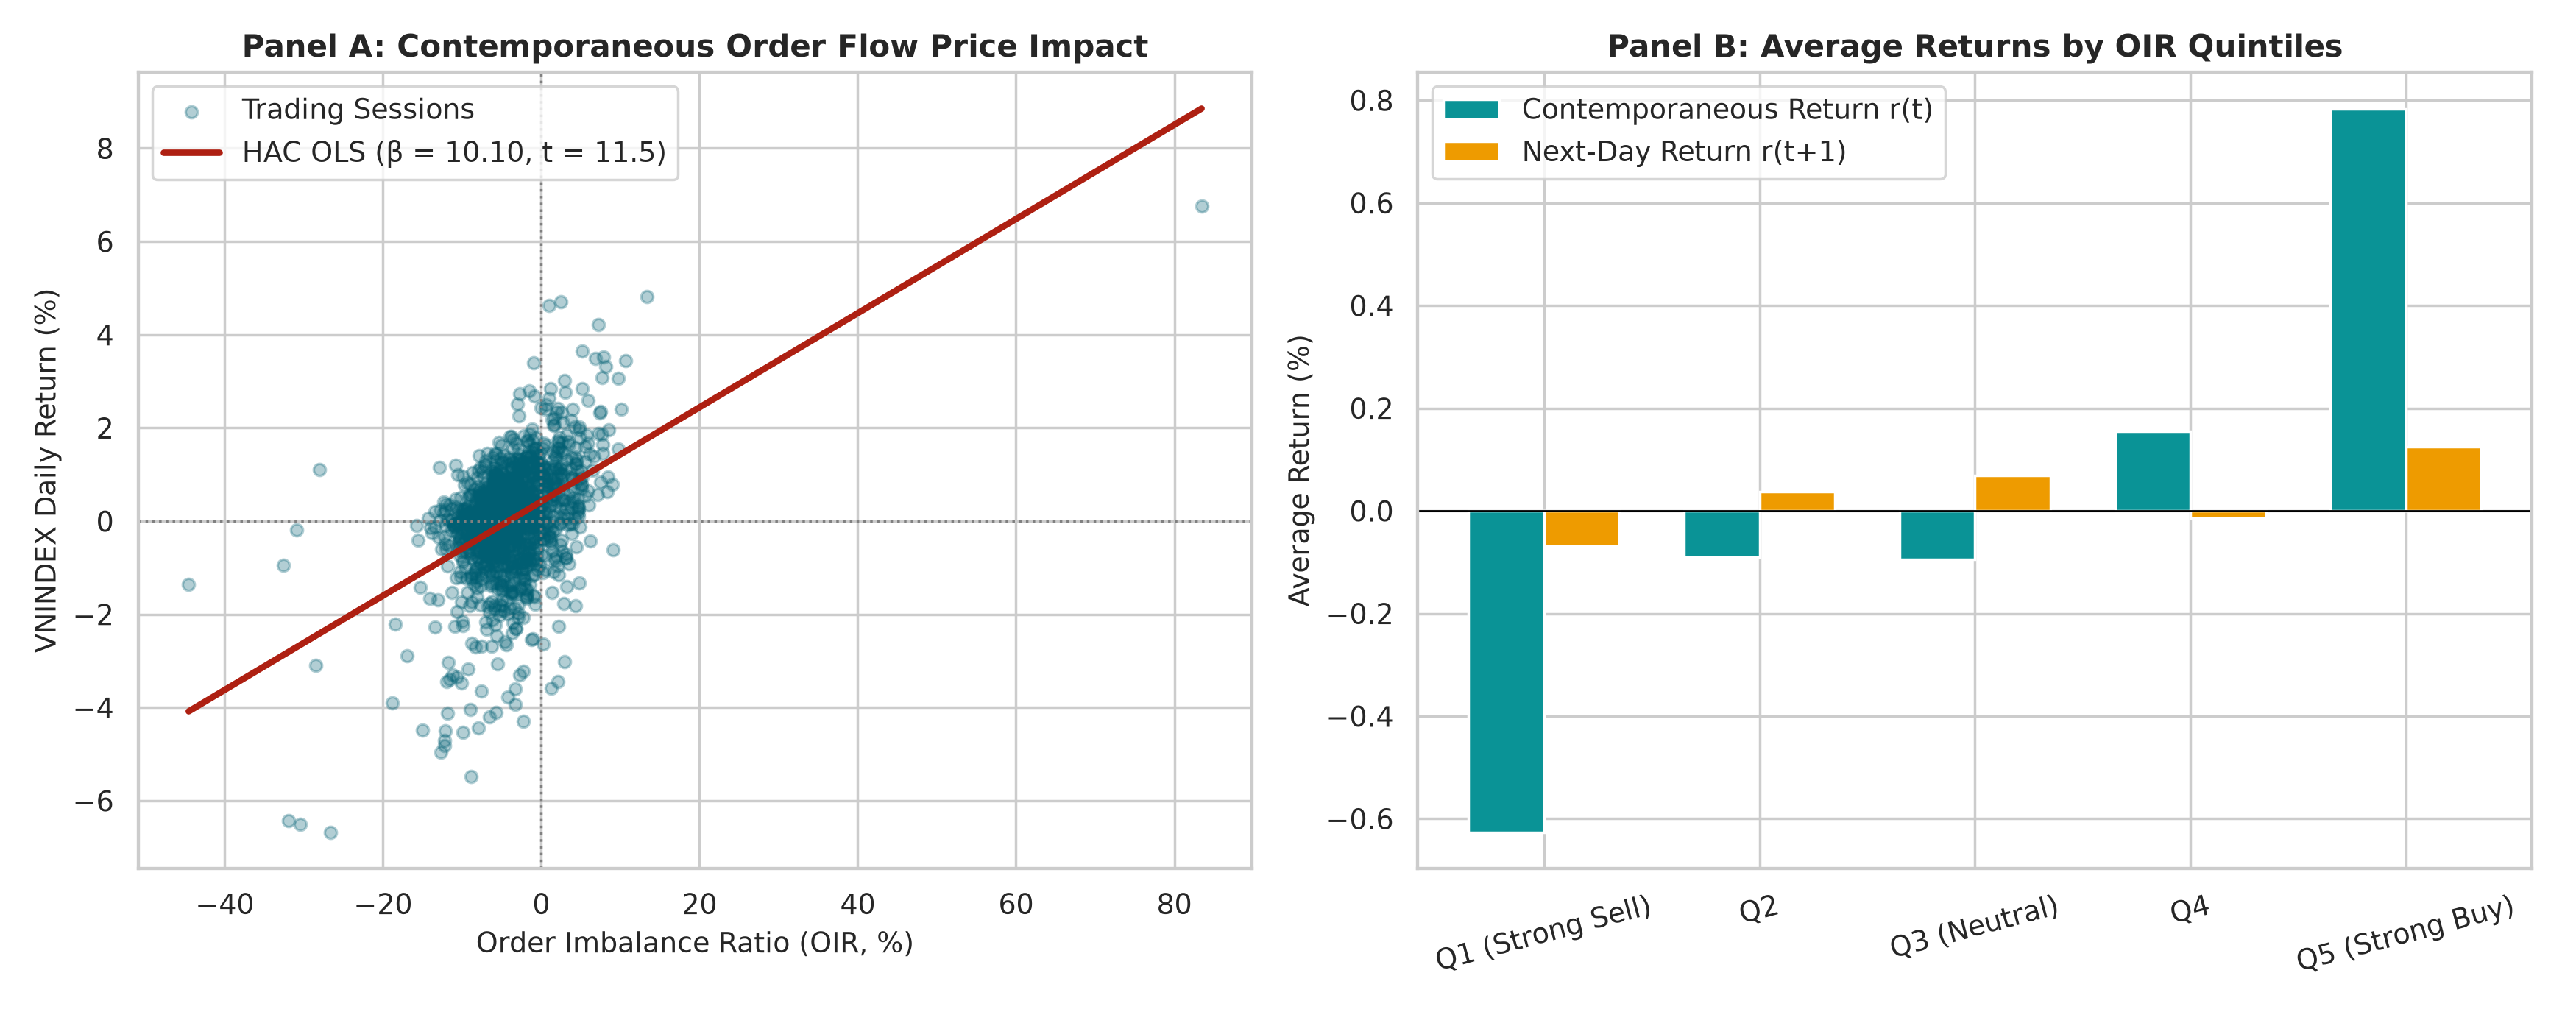
\includegraphics[width=0.95\textwidth]{fig1_order_imbalance_impact.png}
\caption{Order book imbalance dynamics: contemporaneous scatter fit and quintile sort returns.}
\label{fig:order_flow_plot}
\end{figure}

\section{Conclusion and Research Decision}
\label{sec:conclusion}
\noindent \textbf{Research Decision:} \textbf{ACCEPTED for Contemporaneous Price Impact}. Order queue imbalances are absorbed into daily closing prices with high informational efficiency, leaving zero profitable overnight drift.

\bibliographystyle{apalike}
\bibliography{references}
\end{document}
